%\documentclass[12pt]{article}
%\usepackage{ctex} % 中文支持
%\usepackage{titling} % 标题格式定制
%\usepackage{lipsum} % 示例文本
%\usepackage{titlesec} % 标题格式定制
%\usepackage{graphicx}
%
%% 设置标题格式
%\titleformat{\section}{\centering\Large\bfseries}{\thesection}{1em}{}
%\titleformat{\subsection}{\centering\large\bfseries}{\thesubsection}{1em}{}
%\titleformat{\subsubsection}{\centering\normalsize\bfseries}{\thesubsubsection}{1em}{}
%
%% 调整标题位置
%\setlength{\droptitle}{-4cm}

\documentclass[UTF8]{ctexart}
\usepackage{lmodern}
\usepackage{amsmath}
\usepackage{amssymb}
\usepackage{graphicx}
\usepackage{geometry}
\usepackage{xcolor}

\geometry{left=2.18cm,right=2.18cm,top=1.54cm,bottom=2.0cm}
\pagestyle{empty}
\title{\bf 2025秋计算方法--实验报告 \#1}
\author{姓名：金天昊 \quad 学号：PB24000144}
\date{\today}

\begin{document}

%\title{\huge{\textbf{2023秋计算方法-实验报告\#1}}}
%\author{姓名：\underline{   }\hspace{1cm}学号：PB2151xxxx}
\maketitle
运行环境：Windows 11，VSCode，MSVC 19.42.34436

\section*{实验内容与要求}
\begin{itemize}
  \item{\bf 问题1：}
  给定两个函数~$\color{blue}f(x)=\sqrt{x^2+36}-6$~和~$\color{blue}g(x)=\frac{x^2}{\sqrt{x^2+36} + 6},$
{\bf\color{red} 采用单精度}(即float型)进行编程~(注意：开方sqrt(x)等内置函数的输出结果默认是双精度,
需要强制转成单精度), 分别取\\
$\color{blue}x=4^{-1}, 4^{-2}, 4^{-3}, \cdots, 4^{-11}$，
输出相应的函数值~$\color{blue}f(x)$~和~$\color{blue}g(x)$，
计算结果{\bf 保留12位尾数}(用科学计数形式, 参见表1中的数据格式)，比较并分析两种方法得到的计算结果。
你认为哪种方法得到的计算结果更可靠？请给出你的理由或分析。

  \item{\bf 问题2：} 给定如下数据

%%4042.045051380452, 0.000531415926535, -2759471.276702747, -34.64291531266504, \\
%%2755463.874010974, -0.000031415926535, 0.0000557052996742893.每一步的计算结果,

{\bf
4042.045051380452,  0.000531415926535, -2759471.276702747, 0.0000557052996742895, \\
2755463.874010974, -0.000031415926535, -34.64291531256604.}

分别采取以下4种方式求和：

(a) 顺序求和； ~~~~(b) 逆序（从后往前）求和；

(c) 按绝对值从大到小的顺序, 依次求和;
%正数从大到小依次求和，负数从小到大依次求和，然后二者相加；

(d) 按绝对值从小到大的顺序, 依次求和.
%正数从小到大依次求和，负数从大到小依次求和，然后二者相加.

采{\bf\color{red} 用双精度}进行计算，计算结果中的尾数至少保留9位小数(用科学计数形式，比如1.234567899E$-11$).
比较4种方法得到的计算结果；你认为哪种方法得到的计算结果更精确(即误差最小；提示：想办法算出精确值)？
试给出你的理由或分析。


\item{\bf 问题3：~(计算结果保留10位有效数字)}  Let $\bf \color{blue}\pi \approx 3.14159 26535 897932.$
%=3.14159265358979323846264338327950
%$\frac{\pi}{2024}, \frac{\pi}{10}, \frac{\pi}{6}, \frac{\pi}{4}, \frac{\pi}{3}$
\vspace{-0.1in}
\begin{figure}[htb]% 插入两张图片并且并排
	\centering
        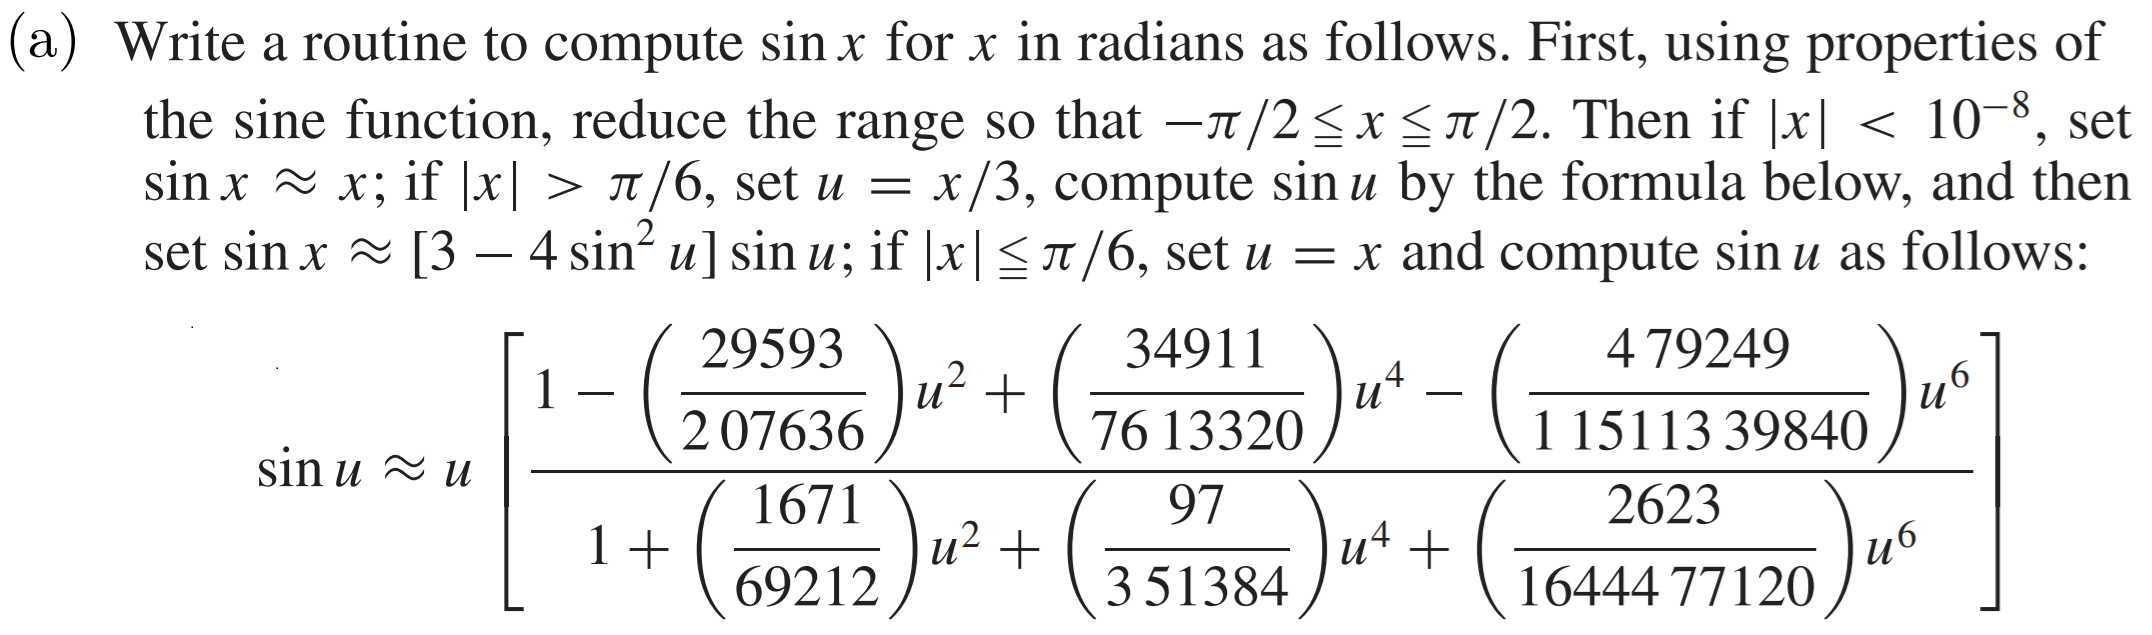
\includegraphics[width=5.80in,height=2.2in, angle=0]{lab01a.png}
  %\caption{\fontsize{9pt}{0pt} N=4 (Left), N=8 (Right)}
\end{figure}

\vspace{-0.1in}
%Compare those results with results obtained by the Taylor formula as  $\color{blue}\sin(x) \approx x- \frac{x^3}{3!} +  \frac{x^5}{5!} - \frac{x^7}{7!}$.
%(a)
(b) Compute $\sin(x)$ by the Taylor approximation formula as $\color{blue}\sin(x) \approx x- \frac{x^3}{3!} +  \frac{x^5}{5!} - \frac{x^7}{7!}$.
\end{itemize}

\clearpage

\section{数值结果（请尽量列表或作图）}
\begin{itemize}
\item 问题1
\begin{table}[htb]
\begin{center}
\begin{tabular}{|c|c|c|} % 3列，每列居中对齐
\hline
$x$ & $\sqrt{x^2+ 36}- 6$ & $ x^2/(\sqrt{x^2+ 36}+ 6)$ \\
\hline
$4^{-1}$=\color{blue}2.500000000000E-01 &\color{blue} 5.206108093262E-03 &\color{blue} 5.206074565649E-03 \\
\hline
$4^{-2}$=6.250000000000E-02  & 3.256797790527E-04 & 3.255119954702E-04 \\
\hline
$4^{-3}$=1.562500000000E-02 & 2.050399780273E-05 & 2.034501630988E-05 \\
\hline
$4^{-4}$=3.906250000000E-03  & 1.430511474609E-06 & 1.271565565730E-06 \\
\hline
$4^{-5}$=9.765625000000E-04  & 0.000000000000E+00 & 7.947286206900E-08 \\
\hline
$4^{-6}$=2.441406250000E-04  & 0.000000000000E+00 & 4.967053879312E-09 \\
\hline
$4^{-7}$=6.103515625000E-05  & 0.000000000000E+00 & 3.104408674570E-10 \\
\hline
$4^{-8}$=1.525878906250E-05  & 0.000000000000E+00 & 1.940255421606E-11 \\
\hline
$4^{-9}$=3.814697265625E-06  & 0.000000000000E+00 & 1.212659638504E-12 \\
\hline
$4^{-10}$=9.536743164062E-07  & 0.000000000000E+00 & 7.579122740650E-14 \\
\hline
$4^{-11}$=2.384185791016E-07  & 0.000000000000E+00 & 4.736951712906E-15 \\
\hline
\end{tabular}
\end{center}
\caption{题1计算结果}
\end{table}


 \item  问题2~(用科学计数形式, 尾数至少保留9位小数)
\begin{table}[htb]
\begin{center}
\small % 缩小字体
\begin{tabular}{|c|c|c|c|c|c|}
\hline
 & 方法(a) & 方法(b) & 方法(c) & 方法(d) & 精确值 \\
\hline
Sum & $1.261923899E-11$ & $-6.821210263E-11$  & $4.684540313E-11$  & $0.000000000E+00$  & $1.856342895E-10$ \\
\hline
\end{tabular}
\end{center}
\caption{题2计算结果}
\end{table}


 \item  问题3~(保留10位有效数字, $\pi \approx 3.14159 26535 897932$)
	\begin{table}[htb]
 \begin{center}
\begin{tabular}{|c|c|c|} % 4列，每列居中对齐  Special Routine
\hline
 $x$  & Formula in 3(a) for $\sin(x)$ & 4-term Taylor Approximation (i.e.,3(b)) for $\sin(x)$  \\
\hline
	$\frac{\pi}{2025}$ & 1.551403157E-03 & 1.551403157E-03 \\
	\hline
	$\frac{\pi}{100}$ & 3.141075908E-02 & 3.141075908E-02 \\ \hline
	$\frac{\pi}{10}$ & 3.090169944E-01 & 3.090169943E-01 \\ \hline
	$\frac{\pi}{6}$  & 5.000000000E-01 & 4.999999919E-01 \\ \hline
	$\frac{\pi}{5}$  & 5.877852523E-01 & 5.877852104E-01 \\ \hline
	$\frac{\pi}{4}$  & 7.071067812E-01 & 7.071064696E-01 \\  \hline
	$\frac{\pi}{3}$  & 8.660254038E-01 & 8.660212717E-01 \\
\hline
\end{tabular}
\end{center}
\caption{题3计算结果}
\end{table}

 %$\frac{\pi}{2024}, \frac{\pi}{10}, \frac{\pi}{6}, \frac{\pi}{4}, \frac{\pi}{3}$

\end{itemize}

\clearpage
\section{算法分析}

\textbf{问题1：}

参照题意实现了两个函数的计算。观察发现，$f(x)$ 在 $x$ 较小时直接变为 $0$，出现了严重的误差，而 $g(x)$ 保持精度较高。整体来看，$g(x)$ 的计算结果更可靠。原因是因为 $x$ 远小于 $6$，$f(x)$ 为两个接近的数相减，在计算机中会出现运算误差。而 $g(x)$ 则避免了这种情况。

\textbf{问题2：}

参照题意实现了四个和的计算方式，并手写小数的高精度计算来求精确值。观察发现，四种方法的计算结果均与精确值有较大差距，但是 (c) 的计算方式误差最小。从计算机运算时，大数与小数相加时，小数部分会被忽略，导致误差的角度分析，理论上 (d) 的计算方式应该误差最小，但是实际计算中发现 (c) 的结果更接近精确值。原因是因为存在两个大数相减，如果使用 (c) 的方式，相当于大数相减的结果被忽略，但是后续较小数的运算不会被忽略，反而 (d) 的方式会导致前面所有的小数运算在进入大数相减时结果被忽略，导致误差更大。

\textbf{问题3：}

参照题意实现了两种 $\sin(x)$ 的计算方式。观察发现，$x$ 较小时，两种方式结果相同，$x$ 较大时，Taylor 公式的结果误差较大。原因是因为 Taylor 公式是对 $\sin(x)$ 的近似，当 $x$ 较大时，近似效果变差。另外 Taylor 公式也会出现大数与小数的计算精度问题。而使用给出的 $x$ 在任意位置拟合精度都较高且对计算机计算友好的公式，能更好地保持精度。
\vspace{3.50cm}

\section{实验小结}

\vspace{0.5cm}

在本次实验中，我通过使用C++程序解决三个数值计算问题，深入理解了数值误差的来源及其影响。通过比较不同计算方法的结果，我认识到选择合适的算法对于提高计算精度的重要性。此外，我还学会了如何在编程中运用不同方法处理浮点数运算，以达到不同程度的误差减少结果。这次实验不仅提升了我的编程技能，也加深了我对数值分析的理解，为今后的学习打下了坚实的基础。

\vspace{2.0cm}


\end{document}
